% Этот шаблон документа разработан в 2014 году
% Данилом Фёдоровых (danil@fedorovykh.ru) 

\documentclass[t, aspectratio=43]{beamer}
\usepackage[]{graphicx}
\usepackage[]{color}
%% maxwidth is the original width if it is less than linewidth
%% otherwise use linewidth (to make sure the graphics do not exceed the margin)
\makeatletter
\def\maxwidth{ %
	\ifdim\Gin@nat@width>\linewidth
	\linewidth
	\else
	\Gin@nat@width
	\fi
}
\makeatother

\definecolor{fgcolor}{rgb}{0.345, 0.345, 0.345}
\newcommand{\hlnum}[1]{\textcolor[rgb]{0.686,0.059,0.569}{#1}}%
\newcommand{\hlstr}[1]{\textcolor[rgb]{0.192,0.494,0.8}{#1}}%
\newcommand{\hlcom}[1]{\textcolor[rgb]{0.678,0.584,0.686}{\textit{#1}}}%
\newcommand{\hlopt}[1]{\textcolor[rgb]{0,0,0}{#1}}%
\newcommand{\hlstd}[1]{\textcolor[rgb]{0.345,0.345,0.345}{#1}}%
\newcommand{\hlkwa}[1]{\textcolor[rgb]{0.161,0.373,0.58}{\textbf{#1}}}%
\newcommand{\hlkwb}[1]{\textcolor[rgb]{0.69,0.353,0.396}{#1}}%
\newcommand{\hlkwc}[1]{\textcolor[rgb]{0.333,0.667,0.333}{#1}}%
\newcommand{\hlkwd}[1]{\textcolor[rgb]{0.737,0.353,0.396}{\textbf{#1}}}%

%\AtBeginSection[]
%{
%	\begin{frame}<beamer>
%		\frametitle{Outline for section \thesection}
%		\tableofcontents[currentsection]
%	\end{frame}
%}

\usepackage{framed}


\definecolor{shadecolor}{rgb}{.97, .97, .97}
\definecolor{messagecolor}{rgb}{0, 0, 0}
\definecolor{warningcolor}{rgb}{1, 0, 1}
\definecolor{errorcolor}{rgb}{1, 0, 0}
\newenvironment{knitrout}{}{} % an empty environment to be redefined in TeX

\usepackage{alltt}  % [t], [c], или [b] --- вертикальное выравнивание на слайдах (верх, центр, низ)
%\documentclass[handout]{beamer} % Раздаточный материал (на слайдах всё сразу)
%\documentclass[aspectratio=169]{beamer} % Соотношение сторон

%\usetheme{Berkeley} % Тема оформления
%\usetheme{Bergen}
%\usetheme{Szeged}

%\usecolortheme{beaver} % Цветовая схема
%\useinnertheme{circles}
%\useinnertheme{rectangles}

%\usetheme{Madrid}
\usetheme{HSE}

%%% Работа с русским языком
\usepackage[cm-default]{fontspec}
\usepackage{xunicode}
\usepackage{xltxtra}
%\usepackage{polyglossia}
%\setdefaultlanguage[spelling=modern]{russian}
%\setotherlanguage{english}

\setmainfont{Times New Roman}
\setsansfont{Arial}
\setmonofont{Inconsolata}

%\usepackage{pscyr}
\usepackage{cmap}					% поиск в PDF
\usepackage{mathtext} 				% русские буквы в формулах
\usepackage[T2A]{fontenc}			% кодировка
\usepackage[utf8]{inputenc}			% кодировка исходного текста
\usepackage[english,russian]{babel}	% локализация и переносы

%% Beamer по-русски
\newtheorem{rtheorem}{Теорема}
\newtheorem{rproof}{Доказательство}
\newtheorem{rexample}{Пример}

%%% Дополнительная работа с математикой
\usepackage{amsmath,amsfonts,amssymb,amsthm,mathtools} % AMS
\usepackage{icomma} % "Умная" запятая: $0,2$ --- число, $0, 2$ --- перечисление

%% Номера формул
%\mathtoolsset{showonlyrefs=true} % Показывать номера только у тех формул, на которые есть \eqref{} в тексте.
%\usepackage{leqno} % Нумерация формул слева

%% Свои команды
\DeclareMathOperator{\sgn}{\mathop{sgn}}

%% Перенос знаков в формулах (по Львовскому)
\newcommand*{\hm}[1]{#1\nobreak\discretionary{}
	{\hbox{$\mathsurround=0pt #1$}}{}}

%%% Работа с картинками
\usepackage{graphicx}  % Для вставки рисунков
\graphicspath{{images/}{images2/}}  % папки с картинками
\setlength\fboxsep{3pt} % Отступ рамки \fbox{} от рисунка
\setlength\fboxrule{1pt} % Толщина линий рамки \fbox{}
\usepackage{wrapfig} % Обтекание рисунков текстом
\usepackage{caption}

\usepackage{pgffor}% http://ctan.org/pkg/pgffor

%%% Работа с таблицами
\usepackage{array,tabularx,tabulary,booktabs} % Дополнительная работа с таблицами
\usepackage{longtable}  % Длинные таблицы
\usepackage{multirow} % Слияние строк в таблице

%%% Программирование
\usepackage{etoolbox} % логические операторы

%%% Другие пакеты
\usepackage{lastpage} % Узнать, сколько всего страниц в документе.
\usepackage{soul} % Модификаторы начертания
\usepackage{csquotes} % Еще инструменты для ссылок
%\usepackage[style=authoryear,maxcitenames=2,backend=biber,sorting=nty]{biblatex}
\usepackage{multicol} % Несколько колонок

%%% Картинки
\usepackage{tikz} % Работа с графикой
\usepackage{pgfplots}
\usepackage{pgfplotstable}

\usepackage{ragged2e}

%
%\usepackage{enumitem}
%\usepackage{tikz}
%\newcommand*\circled[1]{\tikz[baseline=(char.base)]{\node[shape=circle,draw,inner sep=2pt] (char) {#1};}}
%\begin{enumerate}[label=\protect\circled{\arabic*}]



\title{Анализ возрастаний потоков заряженных~частиц в авроральных областях по результатам эксперимента ДЭПРОН}
\subtitle{Семинар НИИЯФ ОКН}
\author[Иван~Золотарев] {И.А. Золотарев, В.В. Бенгин, О.Ю. Нечаев,М.И. Панасюк, В.Л. Петров, И.В. Яшин, Н.Н. Веденкин, А.М. Амелюшкин } 

\date{\today}
\institute[SINP MSU]{Skobeltsyn Institute of Nuclear Physics \\M.V. Lomonosov Moscow State University}












\begin{document}
	
\frame[plain]{\titlepage}	% Титульный слайд


%\begin{frame}{Overview}
%	\tableofcontents
%\end{frame}

%\tableofcontents[h\textsc{}ideallsubsections]

%%%%%%%%%%%%%%%%%%%%%%%%%%%%%%%%%%%%%%%%%%%%%

\section{Всплески интенсивности}\label{header-n0}
\begin{frame}	

\frametitle{\insertsection} 
\begin{figure}
	\centering
	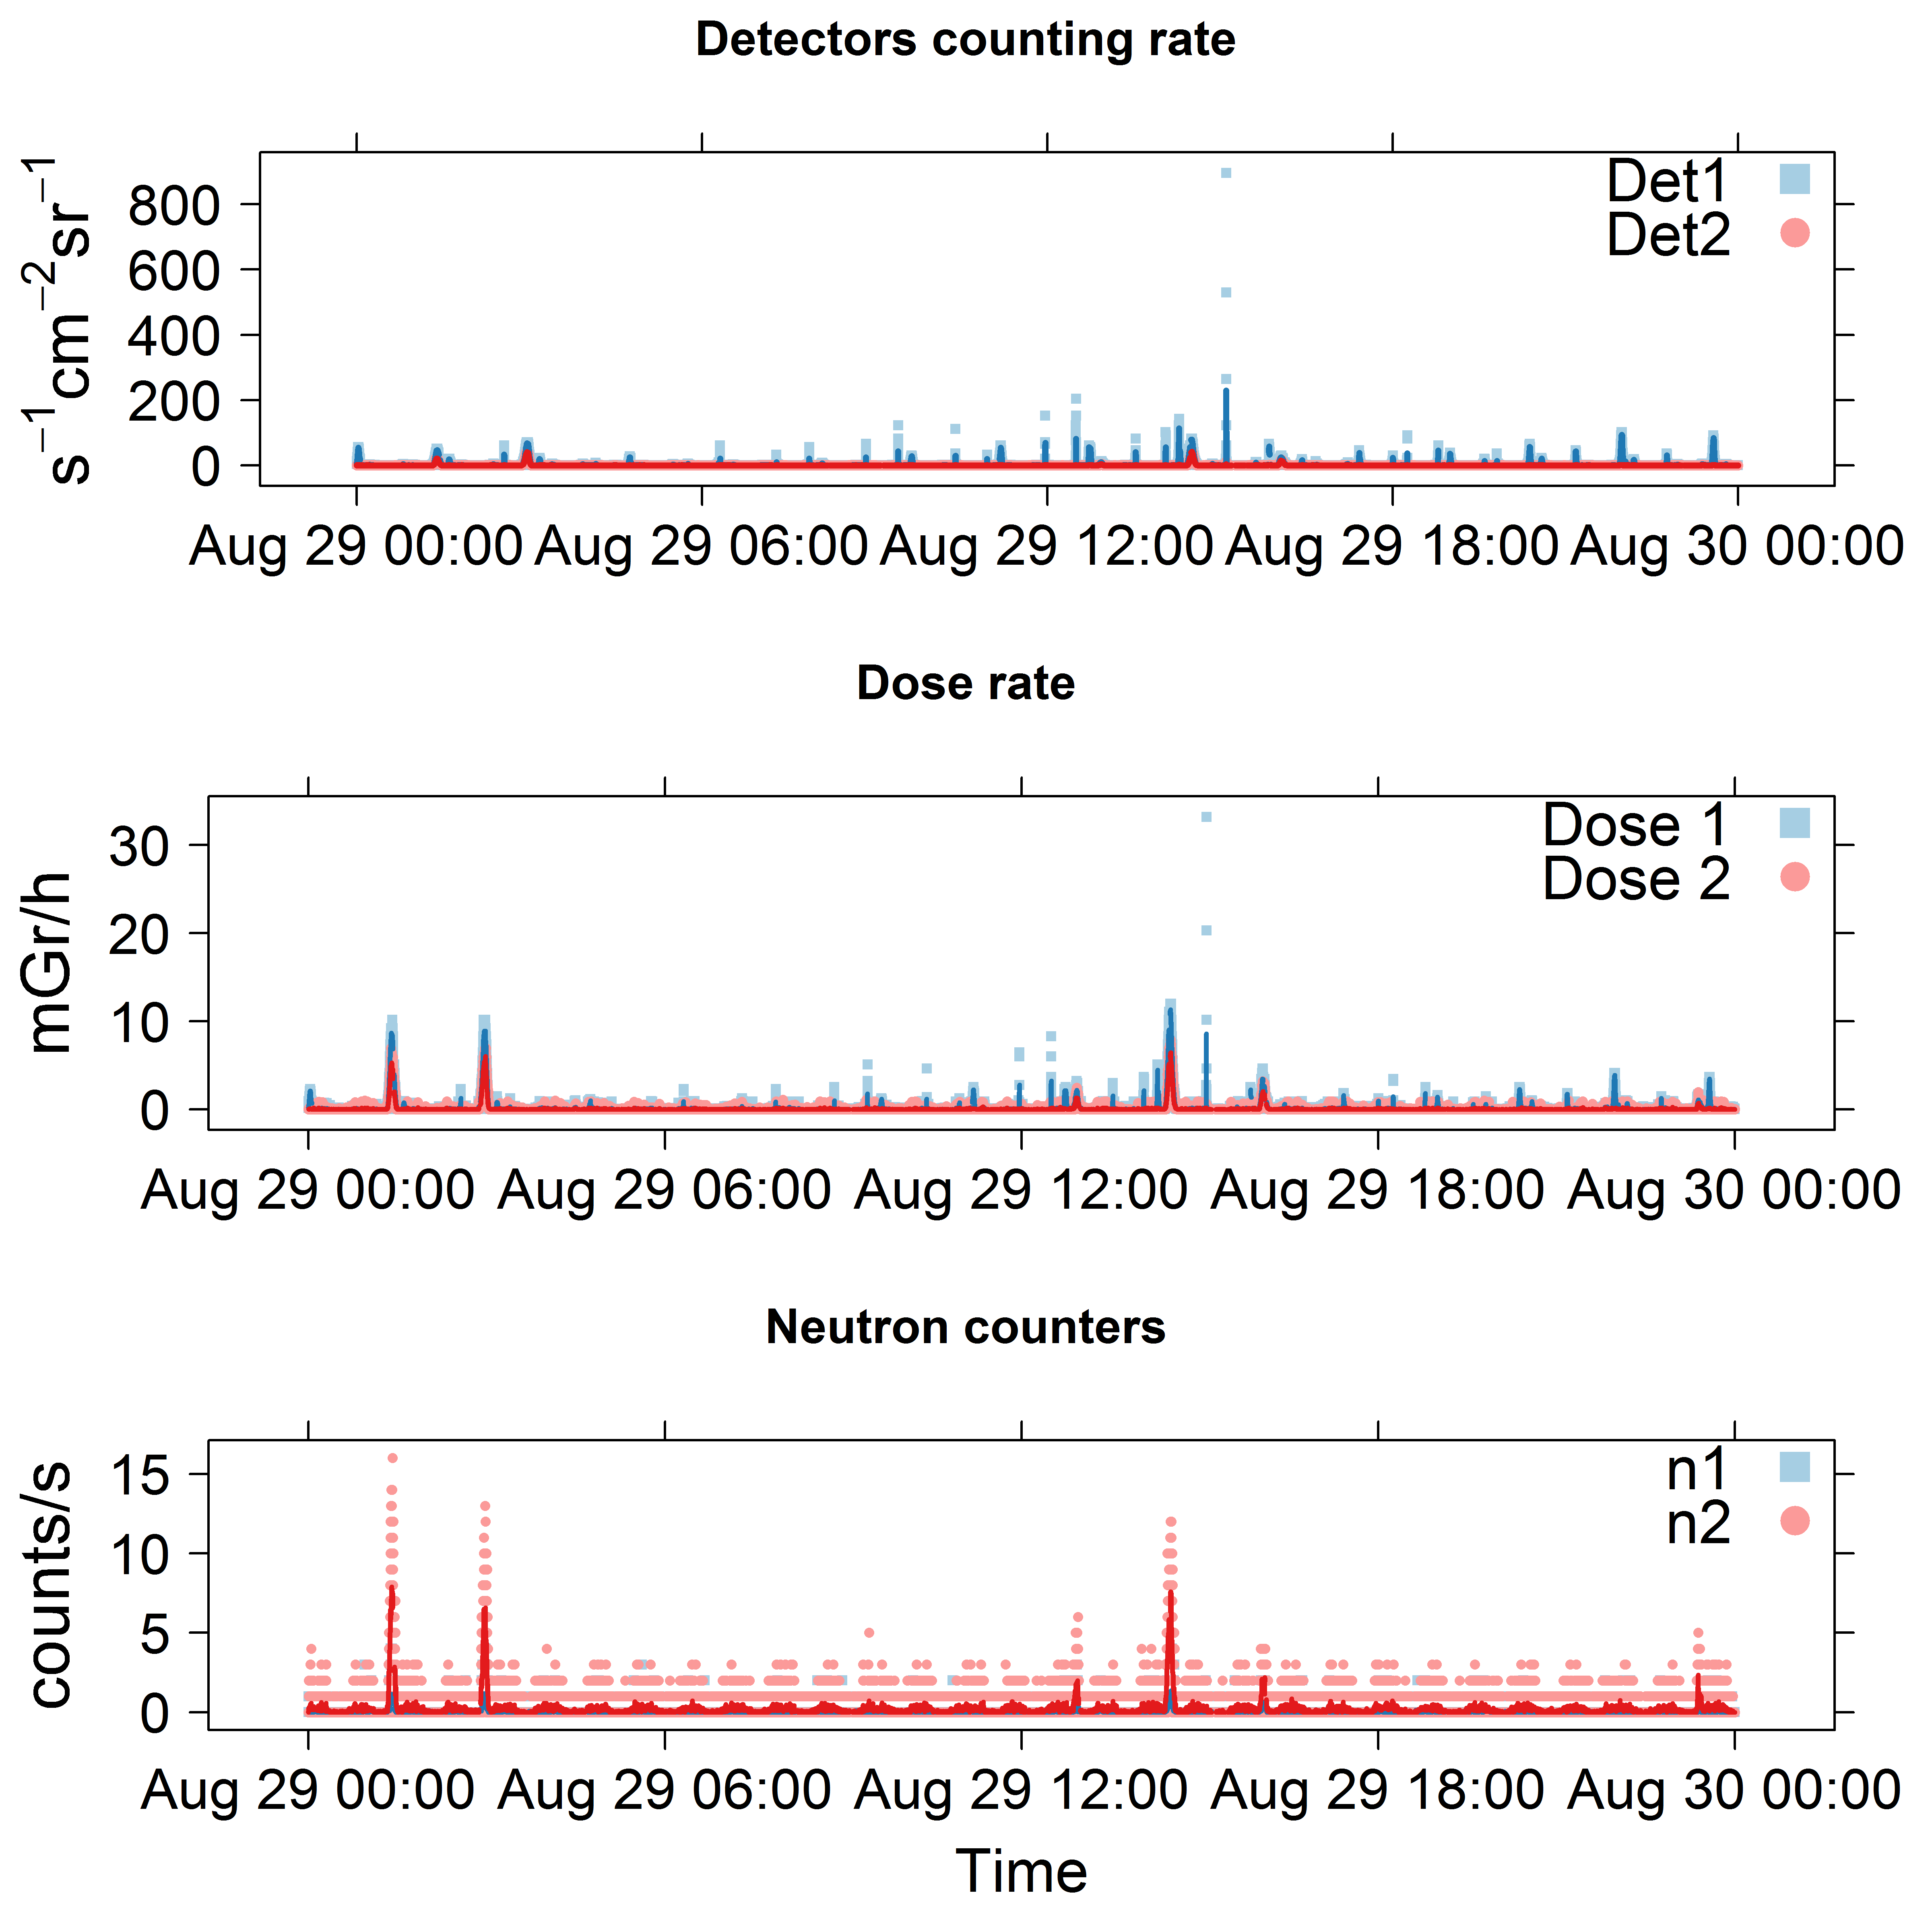
\includegraphics[width=0.6\linewidth]{images/depronseclognew}
	\caption{}
	\label{fig:depronseclognew}
\end{figure}

Временные серии данных показывают всплеск  и прохождение отрогов пояса или
аномалииs
\end{frame}

%%%%%%%%%%%%%%%%%%%%%%%%%%%%%%%%%%%%%%%%%%%%%
\section{История исследования}\label{header-n6}

\begin{frame}	
\frametitle{\insertsection} 

Список характерных публикаций по теме возрастаний потоков частиц в
высокоширотных областях.

\begin{itemize}
	\item
	статья 1962
	\item
	статья 2014
	\item
	статья 2016
\end{itemize}

Новизна нашего исследования заключается в оценке дозиметрических
характеристик всплесков.

\end{frame}

%%%%%%%%%%%%%%%%%%%%%%%%%%%%%%%%%%%%%%%%%%%%%
\section{Кратко по истории вопроса}\label{header-n22}

\begin{frame}	
\frametitle{\insertsection} 

Если кто то из коллег осведомлен о публикациях дозиметрических
характеристик описанных всплесков, мы будем очень благодарны за указание
таких работ.

\end{frame}

%%%%%%%%%%%%%%%%%%%%%%%%%%%%%%%%%%%%%%%%%%%%%
\section{План доклада}\label{header-n26}
\begin{frame}	
\frametitle{\insertsection} 
\begin{enumerate}
	\def\labelenumi{\arabic{enumi}.}
	\item
	Описание прибора ДЭПРОН
	\item
	Алгоритм обработки данных
	\item
	Доступность данных и порядок наземной обработки
	\item
	Результаты без всплесков
	\item
	Статистика всплесков и их феноменология. Критерии отбора событий.
	\item
	Географическое распределение всплесков
	\item
	Связь с параметрами солнечной активности
	\item
	Дозиметрические характеристики всплесков
\end{enumerate}

\end{frame}

%%%%%%%%%%%%%%%%%%%%%%%%%%%%%%%%%%%%%%%%%%%%%
\begin{frame}
\frametitle{Содержание}
\tableofcontents
\end{frame}


\section{ДЭПРОН}
\subsection{Детекторная система}

%%%%%%%%%%%%%%%%%%%%%%%%%%%%%%%%%%%%%%%%%%%%%
\begin{frame}
%\frametitle{\insertsection} 
%\framesubtitle{\insertsubsection}
\begin{columns}[T]
	\begin{column}{.5\textwidth}
		\begin{block}{}
			Коэффициенты перехода от внутренних единиц к потоку и
			дозе. Схема расположения детекторов прибора и защиты вокруг них, минимальные энергии проникающих частиц.
			\begin{enumerate}
				\item Корпус --- 2 мм алюминия, Д16т;
				\item  Бериллиевая бронза --- фольга 10 мкм;
				\item[] Детекторы:
				\begin{enumerate}
					\item[D1] Детектор 	--- 0,3 мм 
					\item[D2] Детектор 	--- 0,3 мм
					\item[D3] \textbf{He-3} счетчик	
					\item[D4] \textbf{He-3} с защитой 1~см оргстекла
				\end{enumerate}
			\end{enumerate}
		\end{block}
	\end{column}
	\begin{column}{.5\textwidth}
		\begin{block}{}
			% Your image included here
			Block diagram
			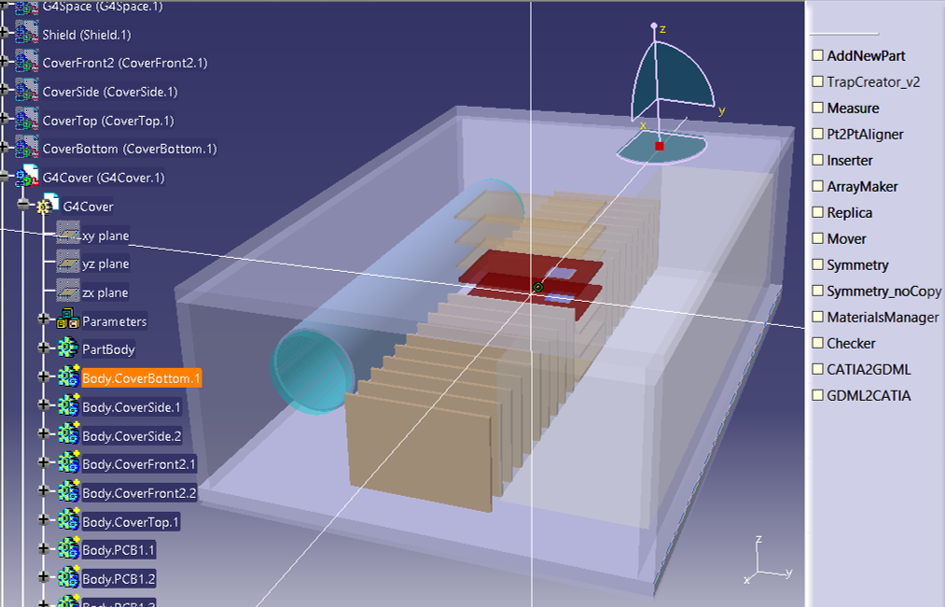
\includegraphics[width=0.8\textwidth]{images/deproncatia2}
		\end{block}
	\end{column}
\end{columns}
\end{frame}

%%%%%%%%%%%%%%%%%%%%%%%%%%%%%%%%%%%%%%%%%%%%%
\begin{frame}
\frametitle{\insertsection} 
\framesubtitle{\insertsubsection}
\begin{columns}[T]
\begin{column}{.5\textwidth}
	\begin{block}{}
		ДЭПРОН - Дозиметр Электронов, ПРОтонов и Нейтральных частиц 	
			
		%DEPRON - Dosimeter of Electrons, PROtons and Neutral particles
		%\includegraphics[width=0.7\linewidth]{images/04062010072}
		{\tiny 
		Наиболее чувствительный информационный параметр при работе ДЭПРОН --- скорость счета детектора 1. Проведем оценку минимальной энергии заряженных частиц, к которым данный детектор чувствителен. Так как детектор закрыт сверху алюминиевой крышкой толщиной 2~мм, он должен быть чувствителен к протонам с энергией больше 20~МэВ и электронам с энергией больше примерно 0,5~МэВ, а также - возможно - к тормозному излучению. Порог дискриминации сигналов с детектора около 100~КэВ. Тем не менее вопрос уточнения границы чувствительности по минимальным энергиям продолжает оставаться важным и на первом этапе были проведены оценки с помощью данных по проникновению электронов и протонов с сайта NIST \cite{NIST}, физическая модель лежащая в основе этих данных основывается на теории Бете\cite{Bethe1930} с поправкой Штернхаймера \cite{Sternheimer1952} на плотность вещества и подробно описана в ряде статей этого института \cite{Bichsel1992, Ashley1972}.
		
		Пользуясь представленными зависимостями, для уточненной минимальной толщины корпуса прибора --- она составляет 2,5~мм, что составляет 0,65~г/см\textsuperscript{2}, была повышена предварительная оценка порога нижних энергий, которые способен регистрировать ДЭПРОН по электронам до 1~МэВ и по протонам до 20~МэВ. Для ядер гелия прибор чувствителен начиная с 90~МэВ. Так как эти зависимости могут использоваться только для средних пробегов частиц, для оценки функции энергетической чувствительности требуется более подробный анализ, который может быть произведен с помощью Монте-Карло моделирования.
	}
	\end{block}
\end{column}
\begin{column}{.5\textwidth}
	\begin{block}{}
		% Your image included here


\begin{figure}[H]
	\centering
	%	\fcolorbox{red}{yellow}{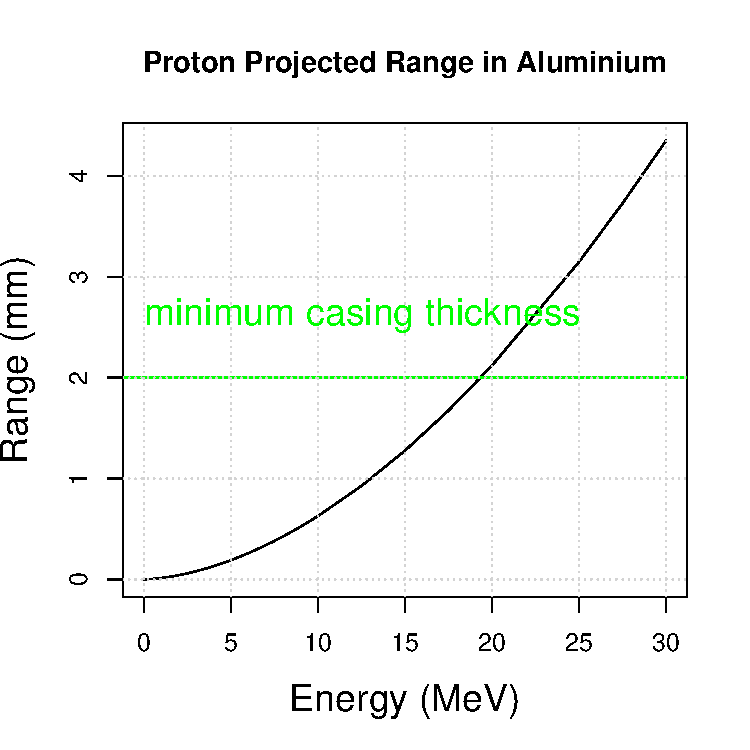
\includegraphics[width=0.6\linewidth]{images/pdata}
	%	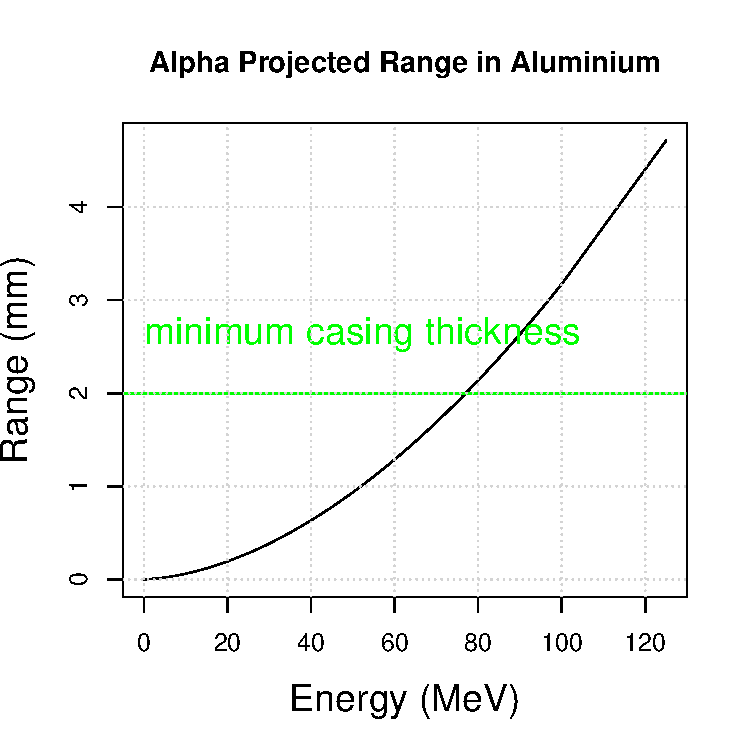
\includegraphics[width=0.6\linewidth]{images/adata}}
	
	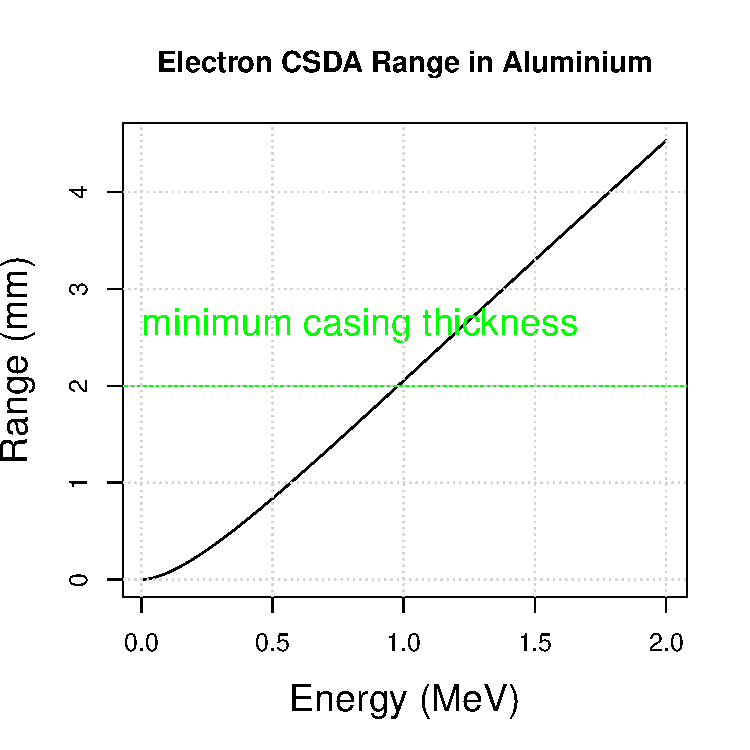
\includegraphics[width=0.32\linewidth]{images/edata}
	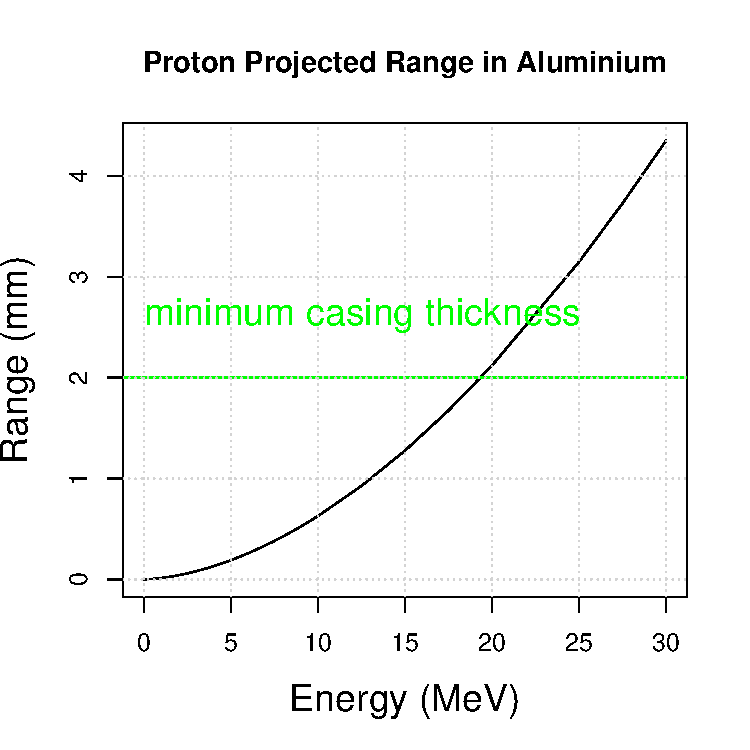
\includegraphics[width=0.32\linewidth]{images/pdata}
	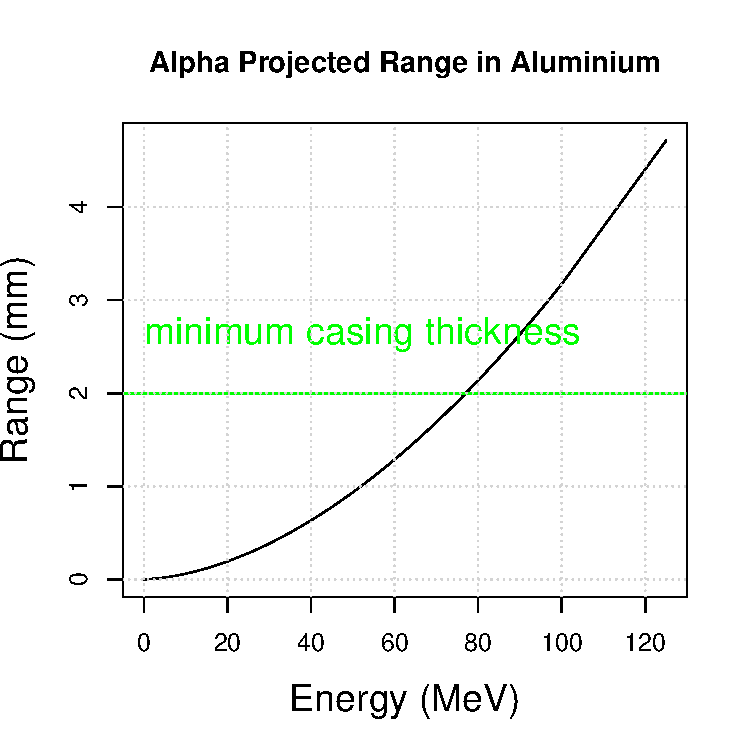
\includegraphics[width=0.32\linewidth]{images/adata}
	\caption{Графики средних пробегов заряженных частиц для алюминия. Представлены величины: ``CSDA range'' --- глубина в приближении непрерывного замедления ``Projected range'' --- среднее значение глубины, на которую заряженная частица проникает в процессе замедления до остановки}
	\label{fig:rplot01}
\end{figure}


	\end{block}
\end{column}
\end{columns}
\end{frame}


%%%%%%%%%%%%%%%%%%%%%%%%%%%%%%%%%%%%%%%%%%%%%
\section{Алгоритм обработки данных}

\begin{frame}	
	\frametitle{\insertsection} 
	\framesubtitle{Особенности алгоритма обработки данных для поиска всплесков}
	
\end{frame}


%%%%%%%%%%%%%%%%%%%%%%%%%%%%%%%%%%%%%%%%%%%%%
\section{Доступность данных}

\begin{frame}	
\frametitle{\insertsection} 
\framesubtitle{Доступность данных и порядок наземной обработки}

\end{frame}

%%%%%%%%%%%%%%%%%%%%%%%%%%%%%%%%%%%%%%%%%%%%%
\section{Результаты без всплесков}

\begin{frame}	
\frametitle{\insertsection} 
\framesubtitle{Особенности алгоритма обработки данных для поиска всплесков}
результаты без всплесков, здесь график рассеяния для аномалии и
полярной области. Скаттерплот: счёт нижнего детектора от счета
верхнего детектора. Ещё по дозе?
\end{frame}

%%%%%%%%%%%%%%%%%%%%%%%%%%%%%%%%%%%%%%%%%%%%%
\section{Статистика всплесков и их феноменология. }

\begin{frame}	
\frametitle{\insertsection} 
\framesubtitle{Критерии отбора событий.}

\end{frame}

%%%%%%%%%%%%%%%%%%%%%%%%%%%%%%%%%%%%%%%%%%%%%
\section{Географическое распределение всплесков}

\begin{frame}	
\frametitle{\insertsection} 


\end{frame}

%%%%%%%%%%%%%%%%%%%%%%%%%%%%%%%%%%%%%%%%%%%%%
\section{Связь с параметрами солнечной активности}

\begin{frame}	
\frametitle{\insertsection} 


\end{frame}
%%%%%%%%%%%%%%%%%%%%%%%%%%%%%%%%%%%%%%%%%%%%%
\section{Дозиметрические характеристики всплесков}

\begin{frame}	
\frametitle{\insertsection} 
\begin{center}
	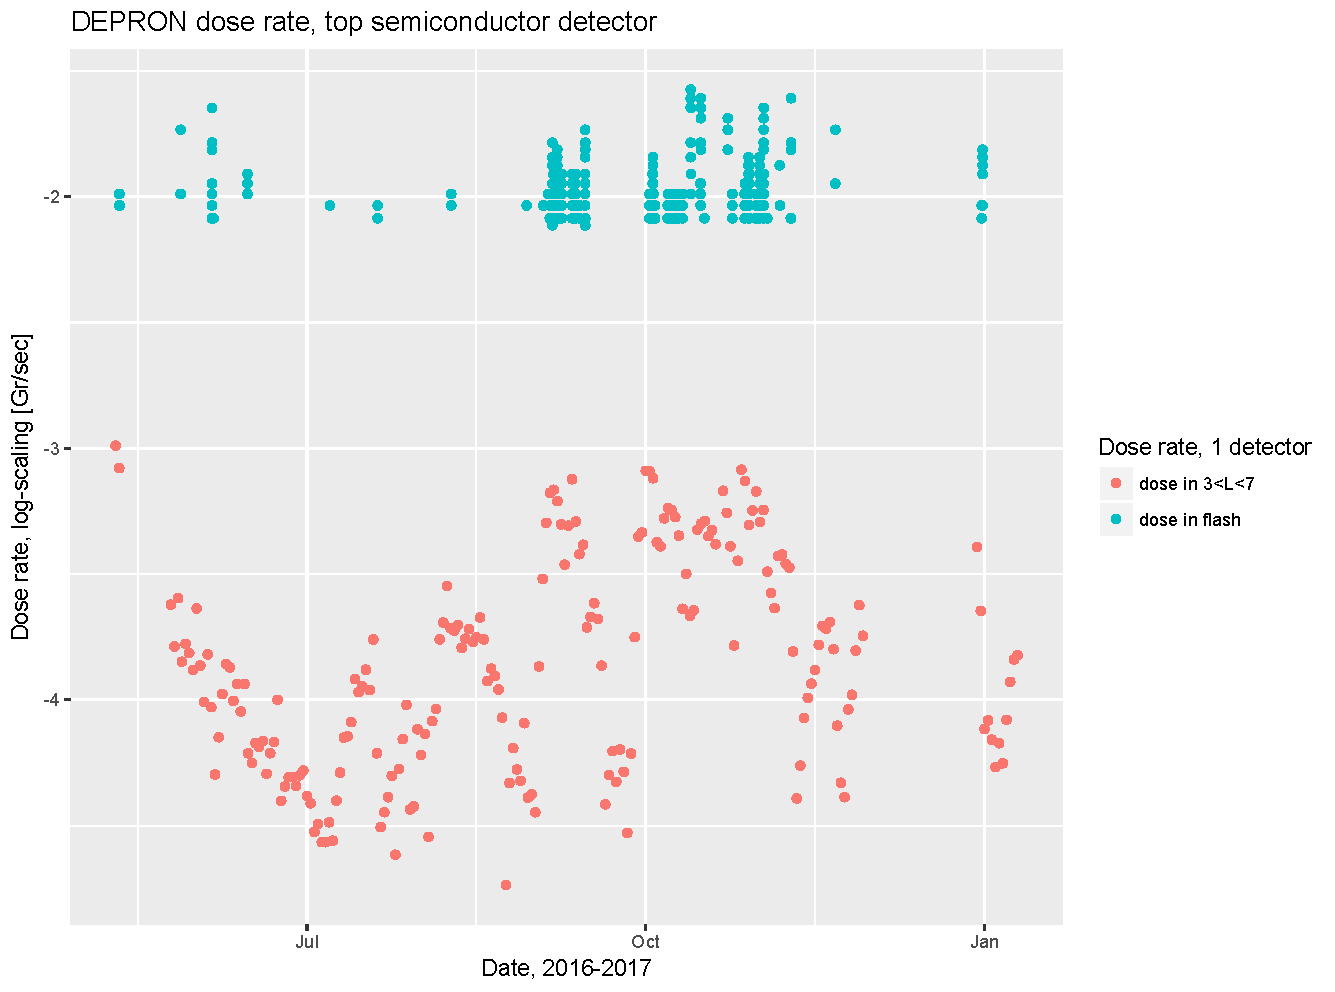
\includegraphics[width=0.5\linewidth]{doseanalisys/flashdose1}
	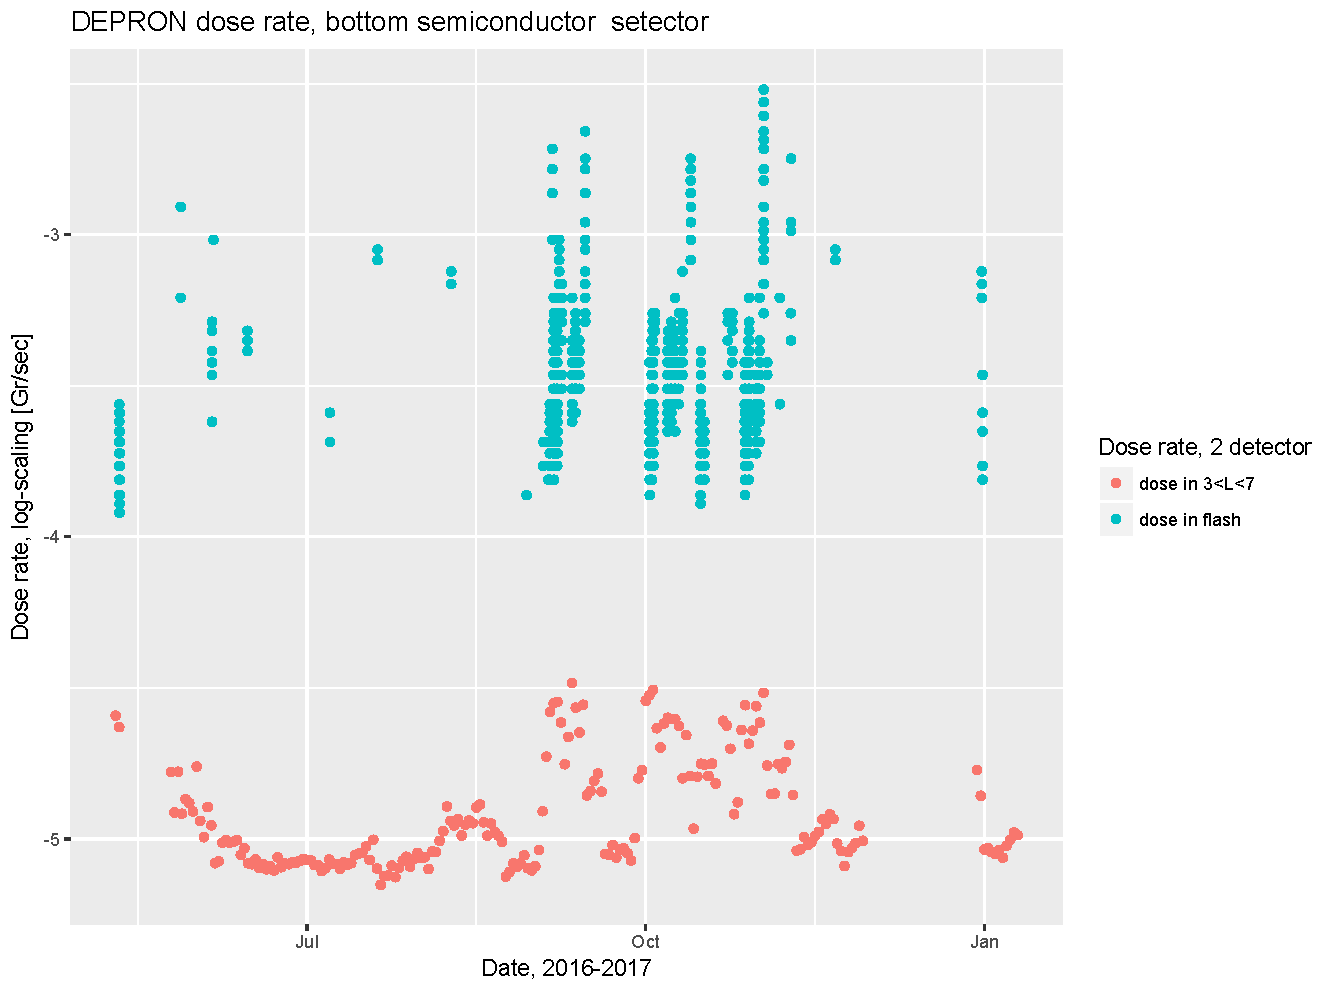
\includegraphics[width=0.5\linewidth]{doseanalisys/flashdose2}
\end{center}


\end{frame}

%%%%%%%%%%%%%%%%%%%%%%%%%%%%%%%%%%%%%%%%%%%%%
\section{Заключение}

\begin{frame}	
\frametitle{\insertsection} 


\end{frame}

\end{document}
%%%%%%%%%%%%%%%%%%%%%%%%%%%%%%%%%%%%%%%%%%%%ы
%%%%%%%%%%%%%%%%%%%%%%%%%%%%%%%%%%%%%%%%%%%%%

\begin{frame}
\frametitle{\insertsection} 
\framesubtitle{\insertsubsection}
\begin{columns}[T]
	\begin{column}{.5\textwidth}
		\begin{block}{}
			
			\begin{figure}
				\centering
				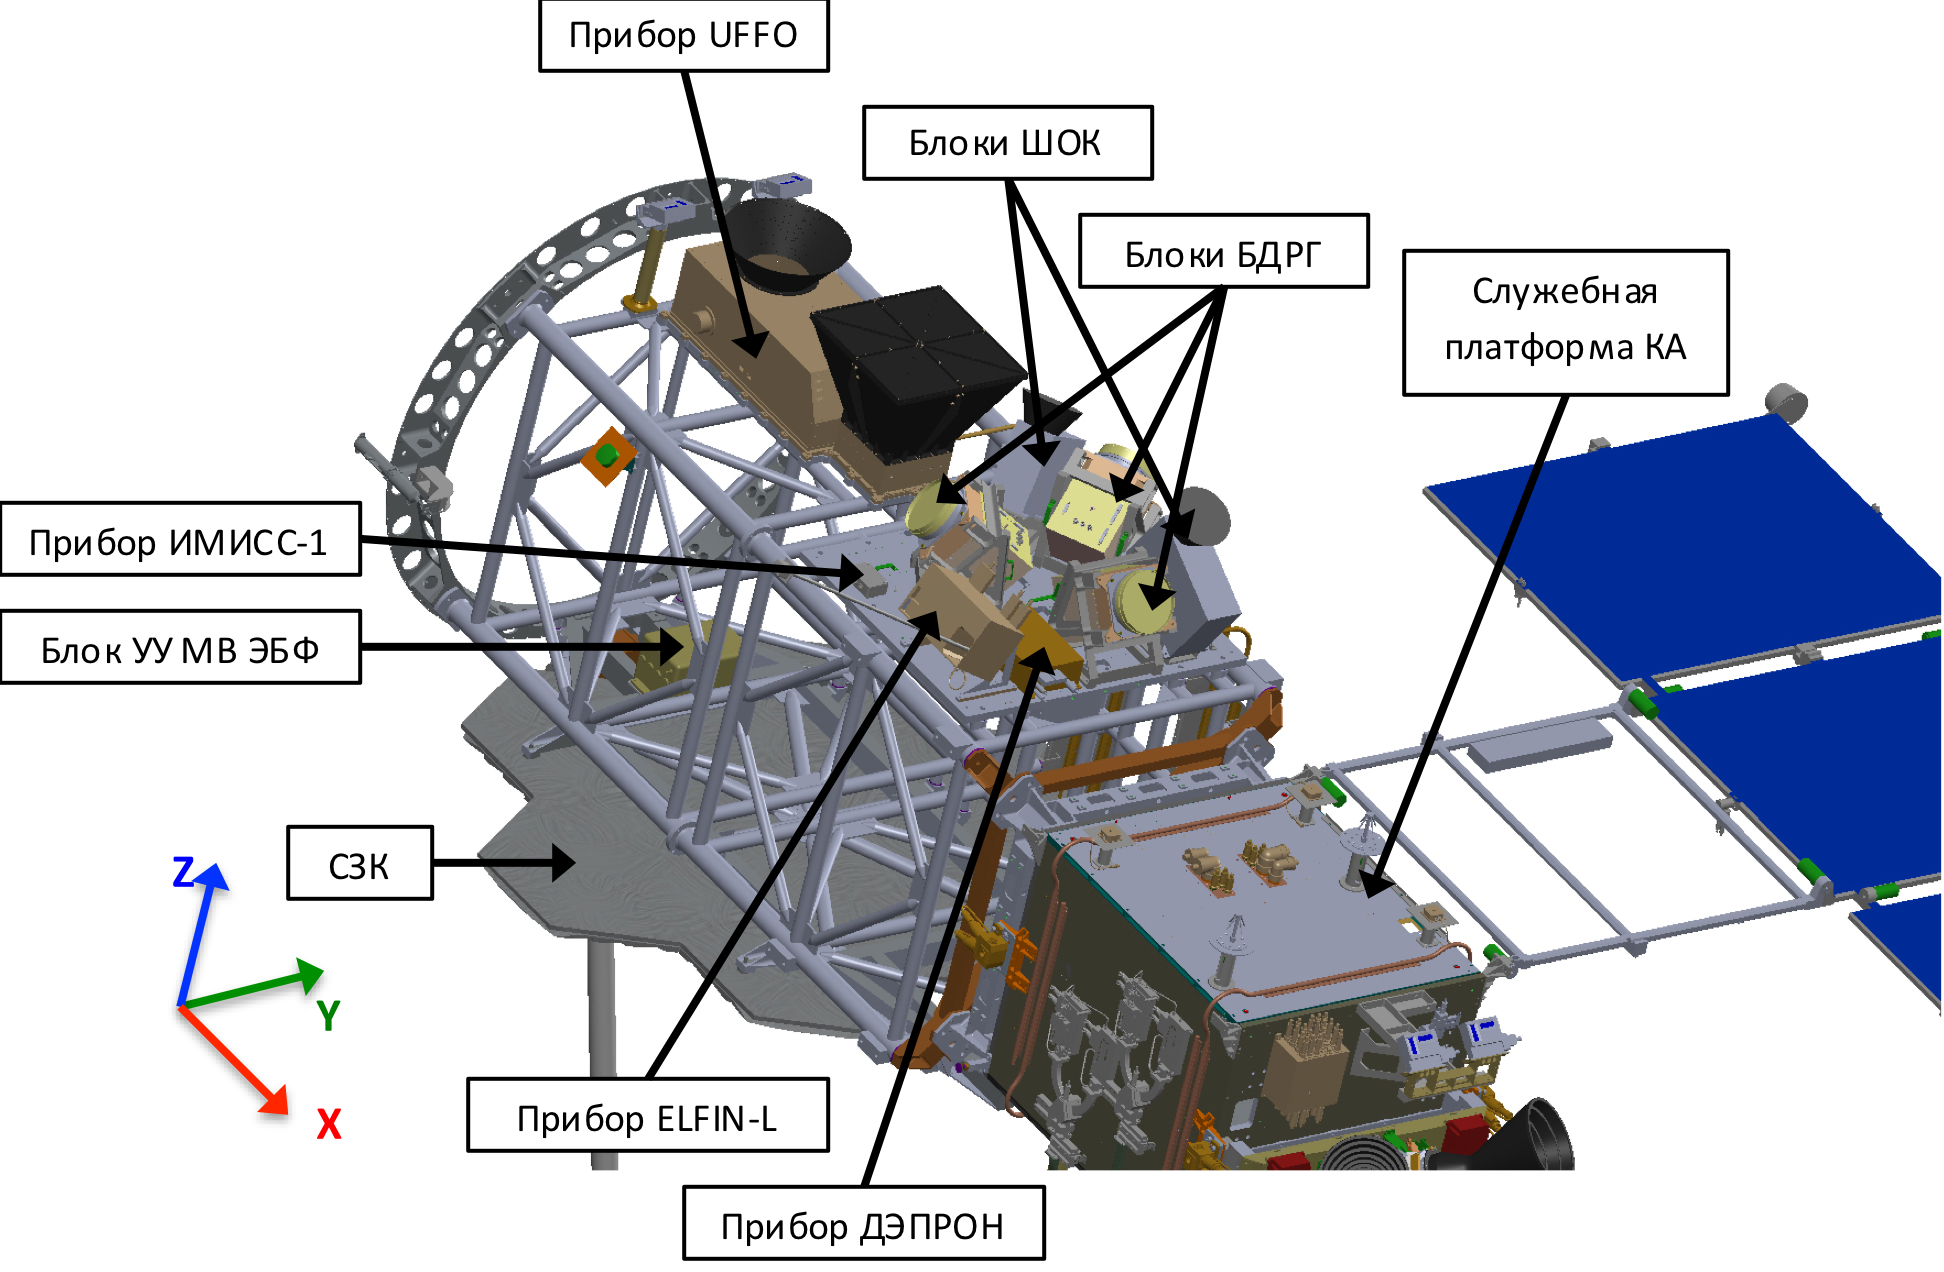
\includegraphics[width=0.9\linewidth]{images/lomo3}
				\caption{Расположение прибора на космическом аппарате}
				\label{fig:lomo3}
			\end{figure}
			
		\end{block}
	\end{column}
	\begin{column}{.5\textwidth}
		\begin{block}{}
			% Your image included here
			
			\begin{figure}
				\centering
				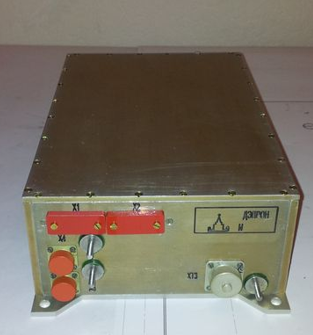
\includegraphics[width=0.6\linewidth]{images/Depronoutside1}
				\caption{}
				\label{fig:depronoutside}
			\end{figure}
			
		\end{block}
	\end{column}
\end{columns}

\end{frame}


%------------------------------------------------		
\section{Dataset}
%------------------------------------------------	
\begin{frame}
	\frametitle{\insertsection} 
	\framesubtitle{\insertsubsection}
	{\small 	
	\justify{
	For the first half of year after the  Lomonosov satellite launch several switching on DEPRON was made according to the mission schedule.
	
	 Now the instrument is working in monitoring mode, with maximum power up time.
	
	During operation of the unit we received 25 thousand data sets containing 100 Mbytes of binary data.	}}

	
	\begin{columns}[T]
		\begin{column}{.5\textwidth}
			\begin{block}{Resulting datasets obtained by decompressing binary data files:}				
			\begin{itemize}
				
				\item  minutes timeseries
				\item  seconds timeseries
				\item  spectra files
				%\item  1 файл массивов высоких амплитуд
				%\item  1 файл массивов нейтронных вспышек
			\end{itemize}
			\end{block}
		\end{column}
		\begin{column}{.5\textwidth}
			\begin{block}{Decoding}
				% Your image included here
				\begin{figure}[th]
					\includegraphics[width=0.6\textwidth]{images/explorer}
				\end{figure}				
			\end{block}
		\end{column}
	\end{columns}
	

	
\end{frame}
	
	

\section{Mission First Results}

\subsection{Time scaling}	
%------------------------------------------------		
\begin{frame}
	\frametitle{\insertsection} 
	\framesubtitle{\insertsubsection}	
	\begin{center}
	
	
\includegraphics[width=0.6\linewidth]{images/screenshot001}

	\includegraphics[width=0.6\linewidth]{images/screenshot002}

	\end{center}
\end{frame}

\subsection{Minute datasets}	
%------------------------------------------------		
\begin{frame}
	\frametitle{\insertsection} 
	\framesubtitle{\insertsubsection}	
	\begin{center}									
		\includegraphics[width=0.65\textwidth]{images/depron_min}%		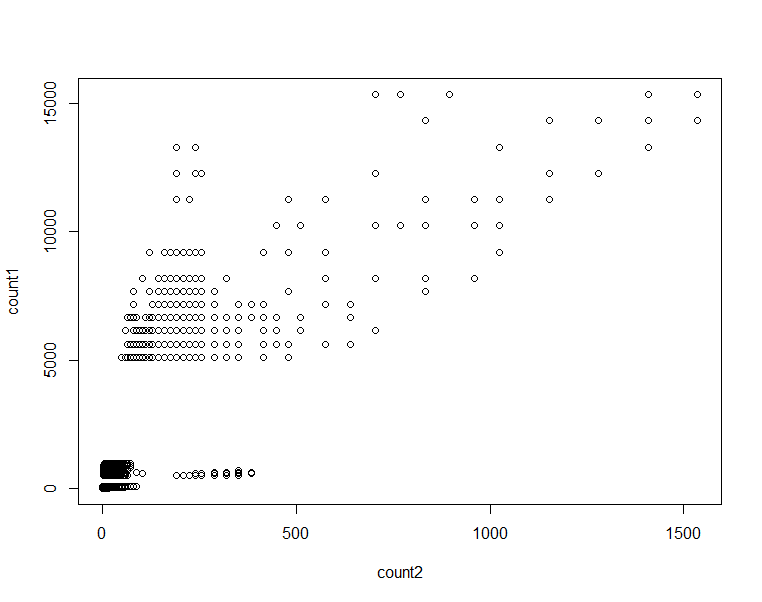
\includegraphics[width=0.8\textwidth]{images/Rplot02}%

		
		{\footnotesize 
		}
	\end{center}
\end{frame}

\subsection{Seconds dataset}	
			
%------------------------------------------------		
\begin{frame}
	\frametitle{\insertsection} 
	\framesubtitle{\insertsubsection}
	\begin{center}									
		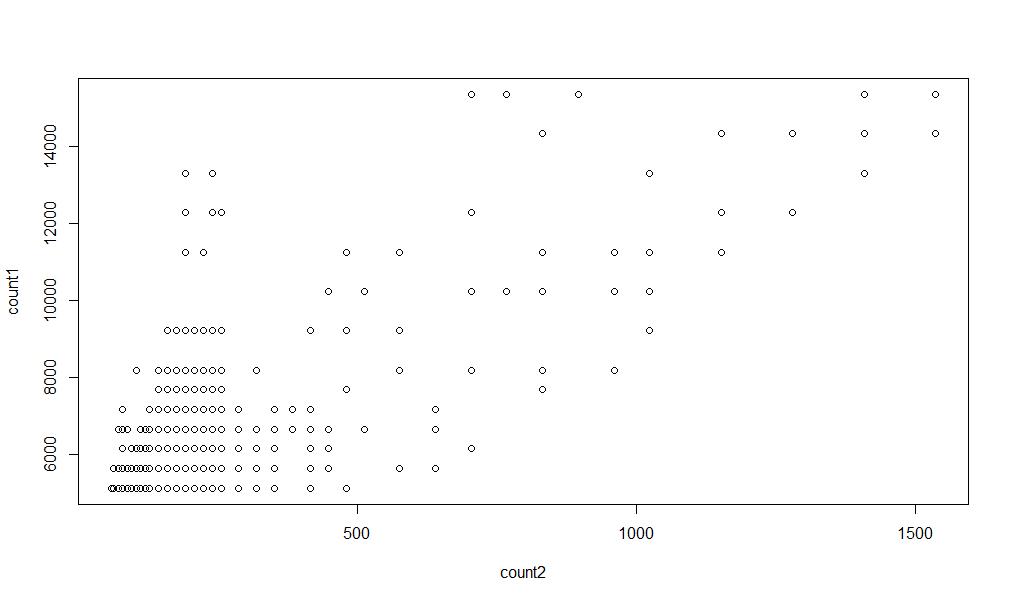
\includegraphics[width=1\textwidth]{images/Rplot05}%
		
		{\footnotesize 
		}
	\end{center}
\end{frame}




\subsection{Anomaly crossing}	
%------------------------------------------------		
\begin{frame}
	\frametitle{\insertsection} 
	\framesubtitle{\insertsubsection}
	\begin{center}		
%		Пример пролета аномалии 
%		кусок траектории с цветом интенсивности
%		Динамика потоков в первом и втором детекторе (без совп)
%		Динамика нейтронных скоростей счета по двум каналам
%		Временные диаграммы				
		
		\begin{columns}[t]
			\column{.5\textwidth}
			\centering
%			\includegraphics[width=5cm,height=4cm]{images/spe1anom}
			\includegraphics[width=5cm,height=4cm]{images/depron_sec_log08-25-16}
			\column{.5\textwidth}
			\centering
			\includegraphics[width=5cm,height=4cm]{images/depron_map_238}\\
			\includegraphics[width=5cm,height=3cm]{images/spe1anom}
		\end{columns}
	\end{center}
\end{frame}

\subsection{South auroral oval crossing}	
%------------------------------------------------		
\begin{frame}
	\frametitle{\insertsection} 
	\framesubtitle{\insertsubsection}
	\begin{center}
%		Пример пролета южной авроральной зоны
%		кусок траектории с цветом интенсивности
%		Динамика потоков в первом и втором детекторе (без совп)
%		Динамика нейтронных скоростей счета по двум каналам
%		Спектр энерговыделения за этот же промежуток времени.
%		Временные диаграммы									
		
		\begin{columns}[t]
			\column{.5\textwidth}
			\centering
%			\includegraphics[width=5cm,height=3.5cm]{images/spe1polar}\\
			\includegraphics[width=5cm,height=4cm]{images/depron_sec_log08-21-1611-35-00}
			\column{.5\textwidth}
			\centering
			\includegraphics[width=5cm,height=4cm]{images/depron_map_234}\\
			\includegraphics[width=5cm,height=3cm]{images/spe1polar}
		\end{columns}
	\end{center}
\end{frame}

\subsection{Timeseries}	
%------------------------------------------------		
\begin{frame}
	\frametitle{\insertsection} 
	\framesubtitle{\insertsubsection}
	\begin{center}		
								
		\includegraphics[width=0.8\textwidth]{images/sec_anom}%
		
		{\footnotesize 
		}
	\end{center}
\end{frame}


\subsection{22 23 августа 2016}
%------------------------------------------------		
\begin{frame}
	\frametitle{\insertsection} 
	\framesubtitle{\insertsubsection}
	Временные диаграммы за периоды 21 и 23 августа (данные левого рисунка заканчиваются в 7:30 22 августа)
	
	\begin{center}									
		\includegraphics[width=0.6\textwidth]{images/image4}%
		
		{\footnotesize 
		}
	\end{center}
\end{frame}

\subsection{20 августа 2016}	
%------------------------------------------------		
\begin{frame}
	\frametitle{\insertsection} 
	\framesubtitle{\insertsubsection}
\begin{center}		
	
	\includegraphics[width=0.8\textwidth]{images/image8}
	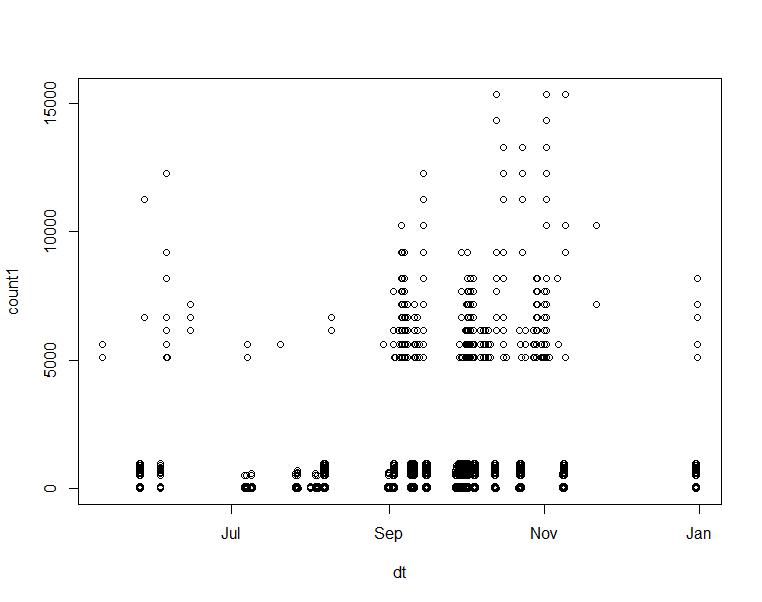
\includegraphics[width=0.2\linewidth]{images/Rplot}
\end{center}
\end{frame}
	

\subsection{21 августа 2016}	
%------------------------------------------------		
\begin{frame}
	\frametitle{\insertsection} 
	\framesubtitle{\insertsubsection}
\begin{center}		
	
	\includegraphics[width=0.8\textwidth]{images/image10}
	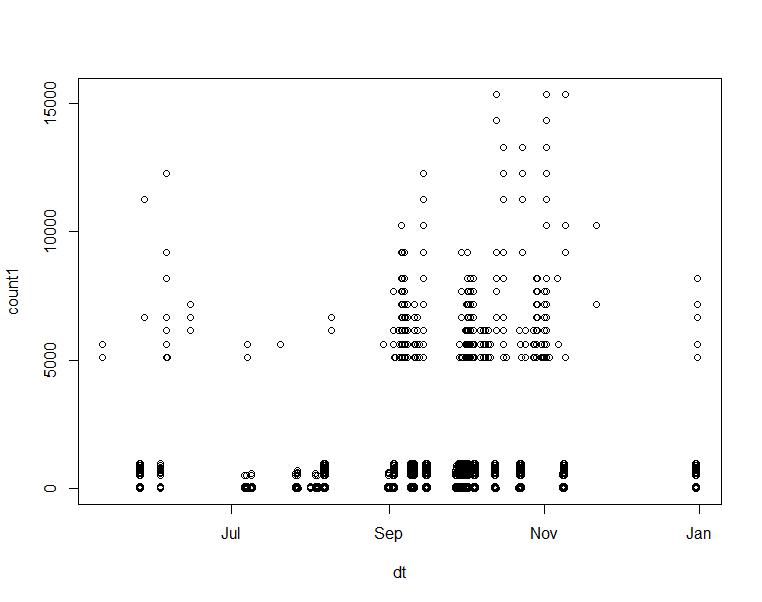
\includegraphics[width=0.2\linewidth]{images/Rplot}
\end{center}
\end{frame}
	

\subsection{23 августа 2016}	
%------------------------------------------------		
\begin{frame}
	\frametitle{\insertsection} 
	\framesubtitle{\insertsubsection}
\begin{center}		
	
	\includegraphics[width=0.8\textwidth]{images/image12}
	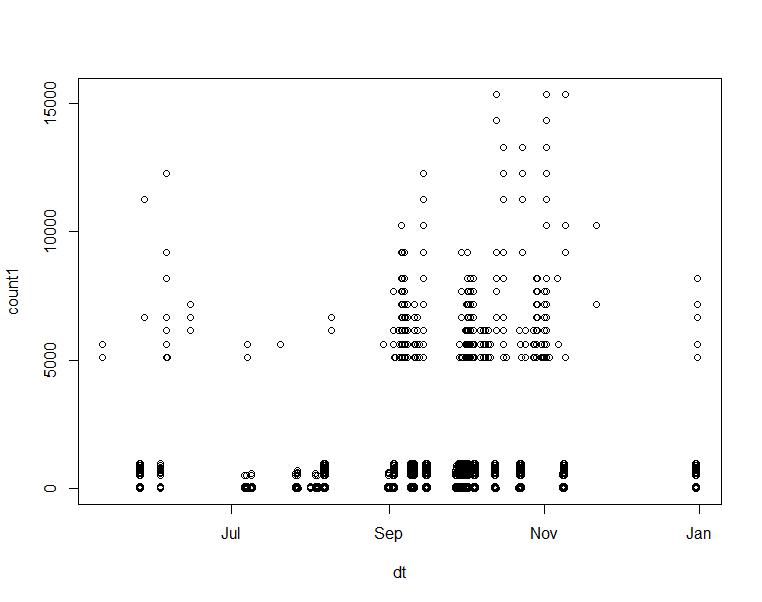
\includegraphics[width=0.2\linewidth]{images/Rplot}
\end{center}
\end{frame}

%------------------------------------------------		
\begin{frame}
	\frametitle{\insertsection} 
	\framesubtitle{\insertsubsection}
	\begin{center}		
		
		\includegraphics[width=0.8\textwidth]{images/image9}
		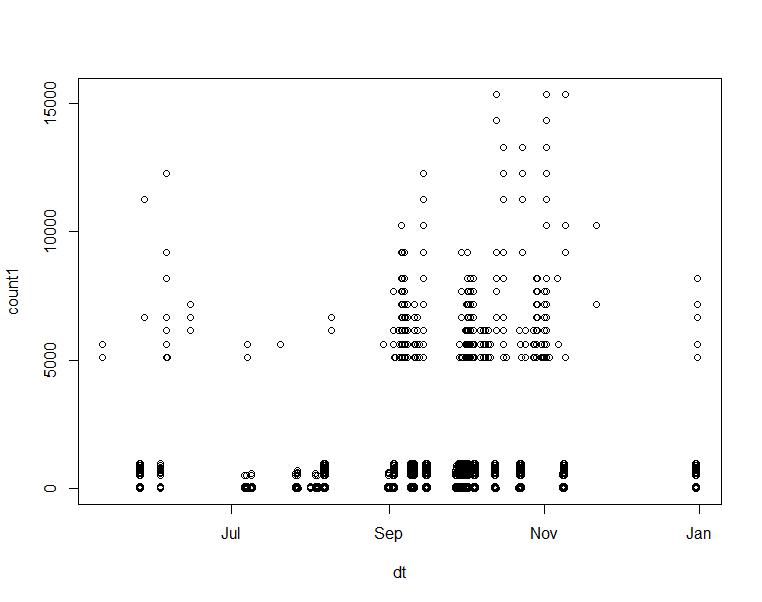
\includegraphics[width=0.2\linewidth]{images/Rplot}
	\end{center}
\end{frame}

%------------------------------------------------		
\begin{frame}
	\frametitle{\insertsection} 
	\framesubtitle{\insertsubsection}
	
	\begin{center}		
		
		\includegraphics[width=0.8\textwidth]{images/image11}
		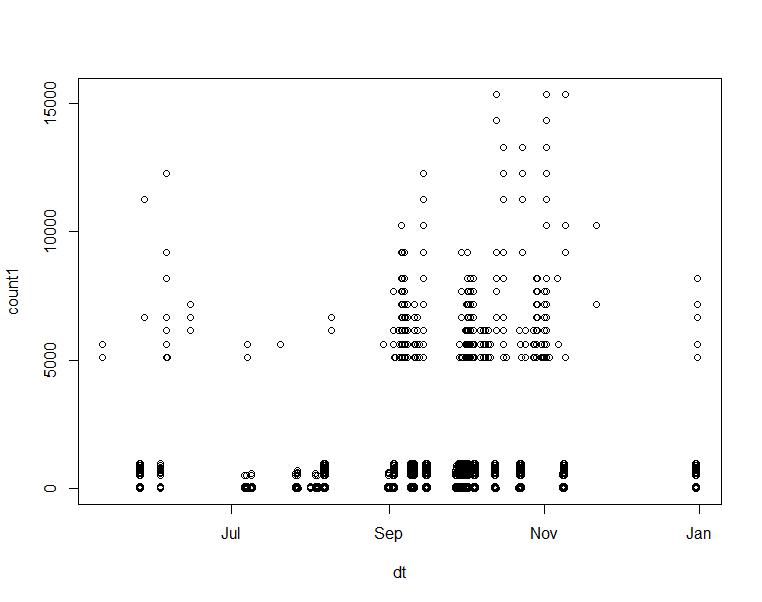
\includegraphics[width=0.2\linewidth]{images/Rplot}
	\end{center}
\end{frame}	
%------------------------------------------------		
\begin{frame}
	\frametitle{\insertsection} 
	\framesubtitle{\insertsubsection}
\begin{center}		
	
	\includegraphics[width=0.8\textwidth]{images/image13}
	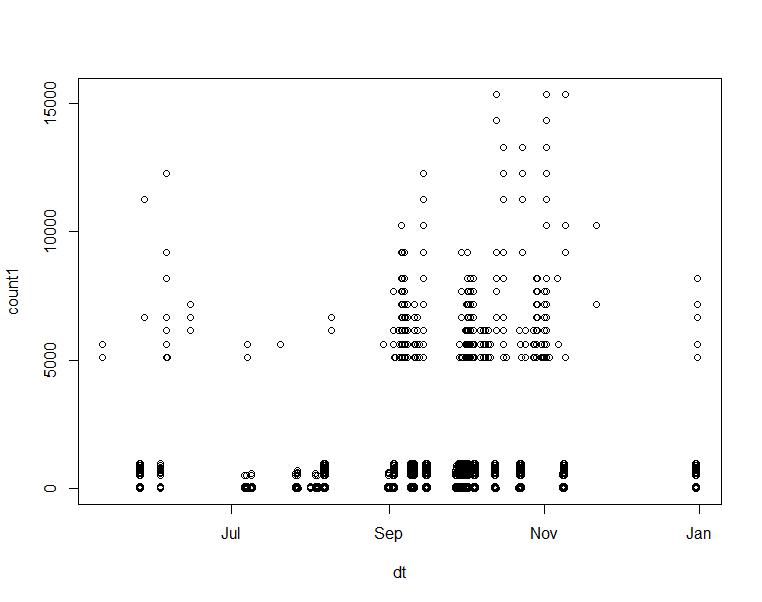
\includegraphics[width=0.2\textwidth]{images/Rplot}
\end{center}
\end{frame}


\subsection{Global Maps}	
%------------------------------------------------		
\begin{frame}
	\frametitle{\insertsection} 
	\framesubtitle{\insertsubsection}
	\begin{center}		
		\rotatebox{90}{Latitude}~
		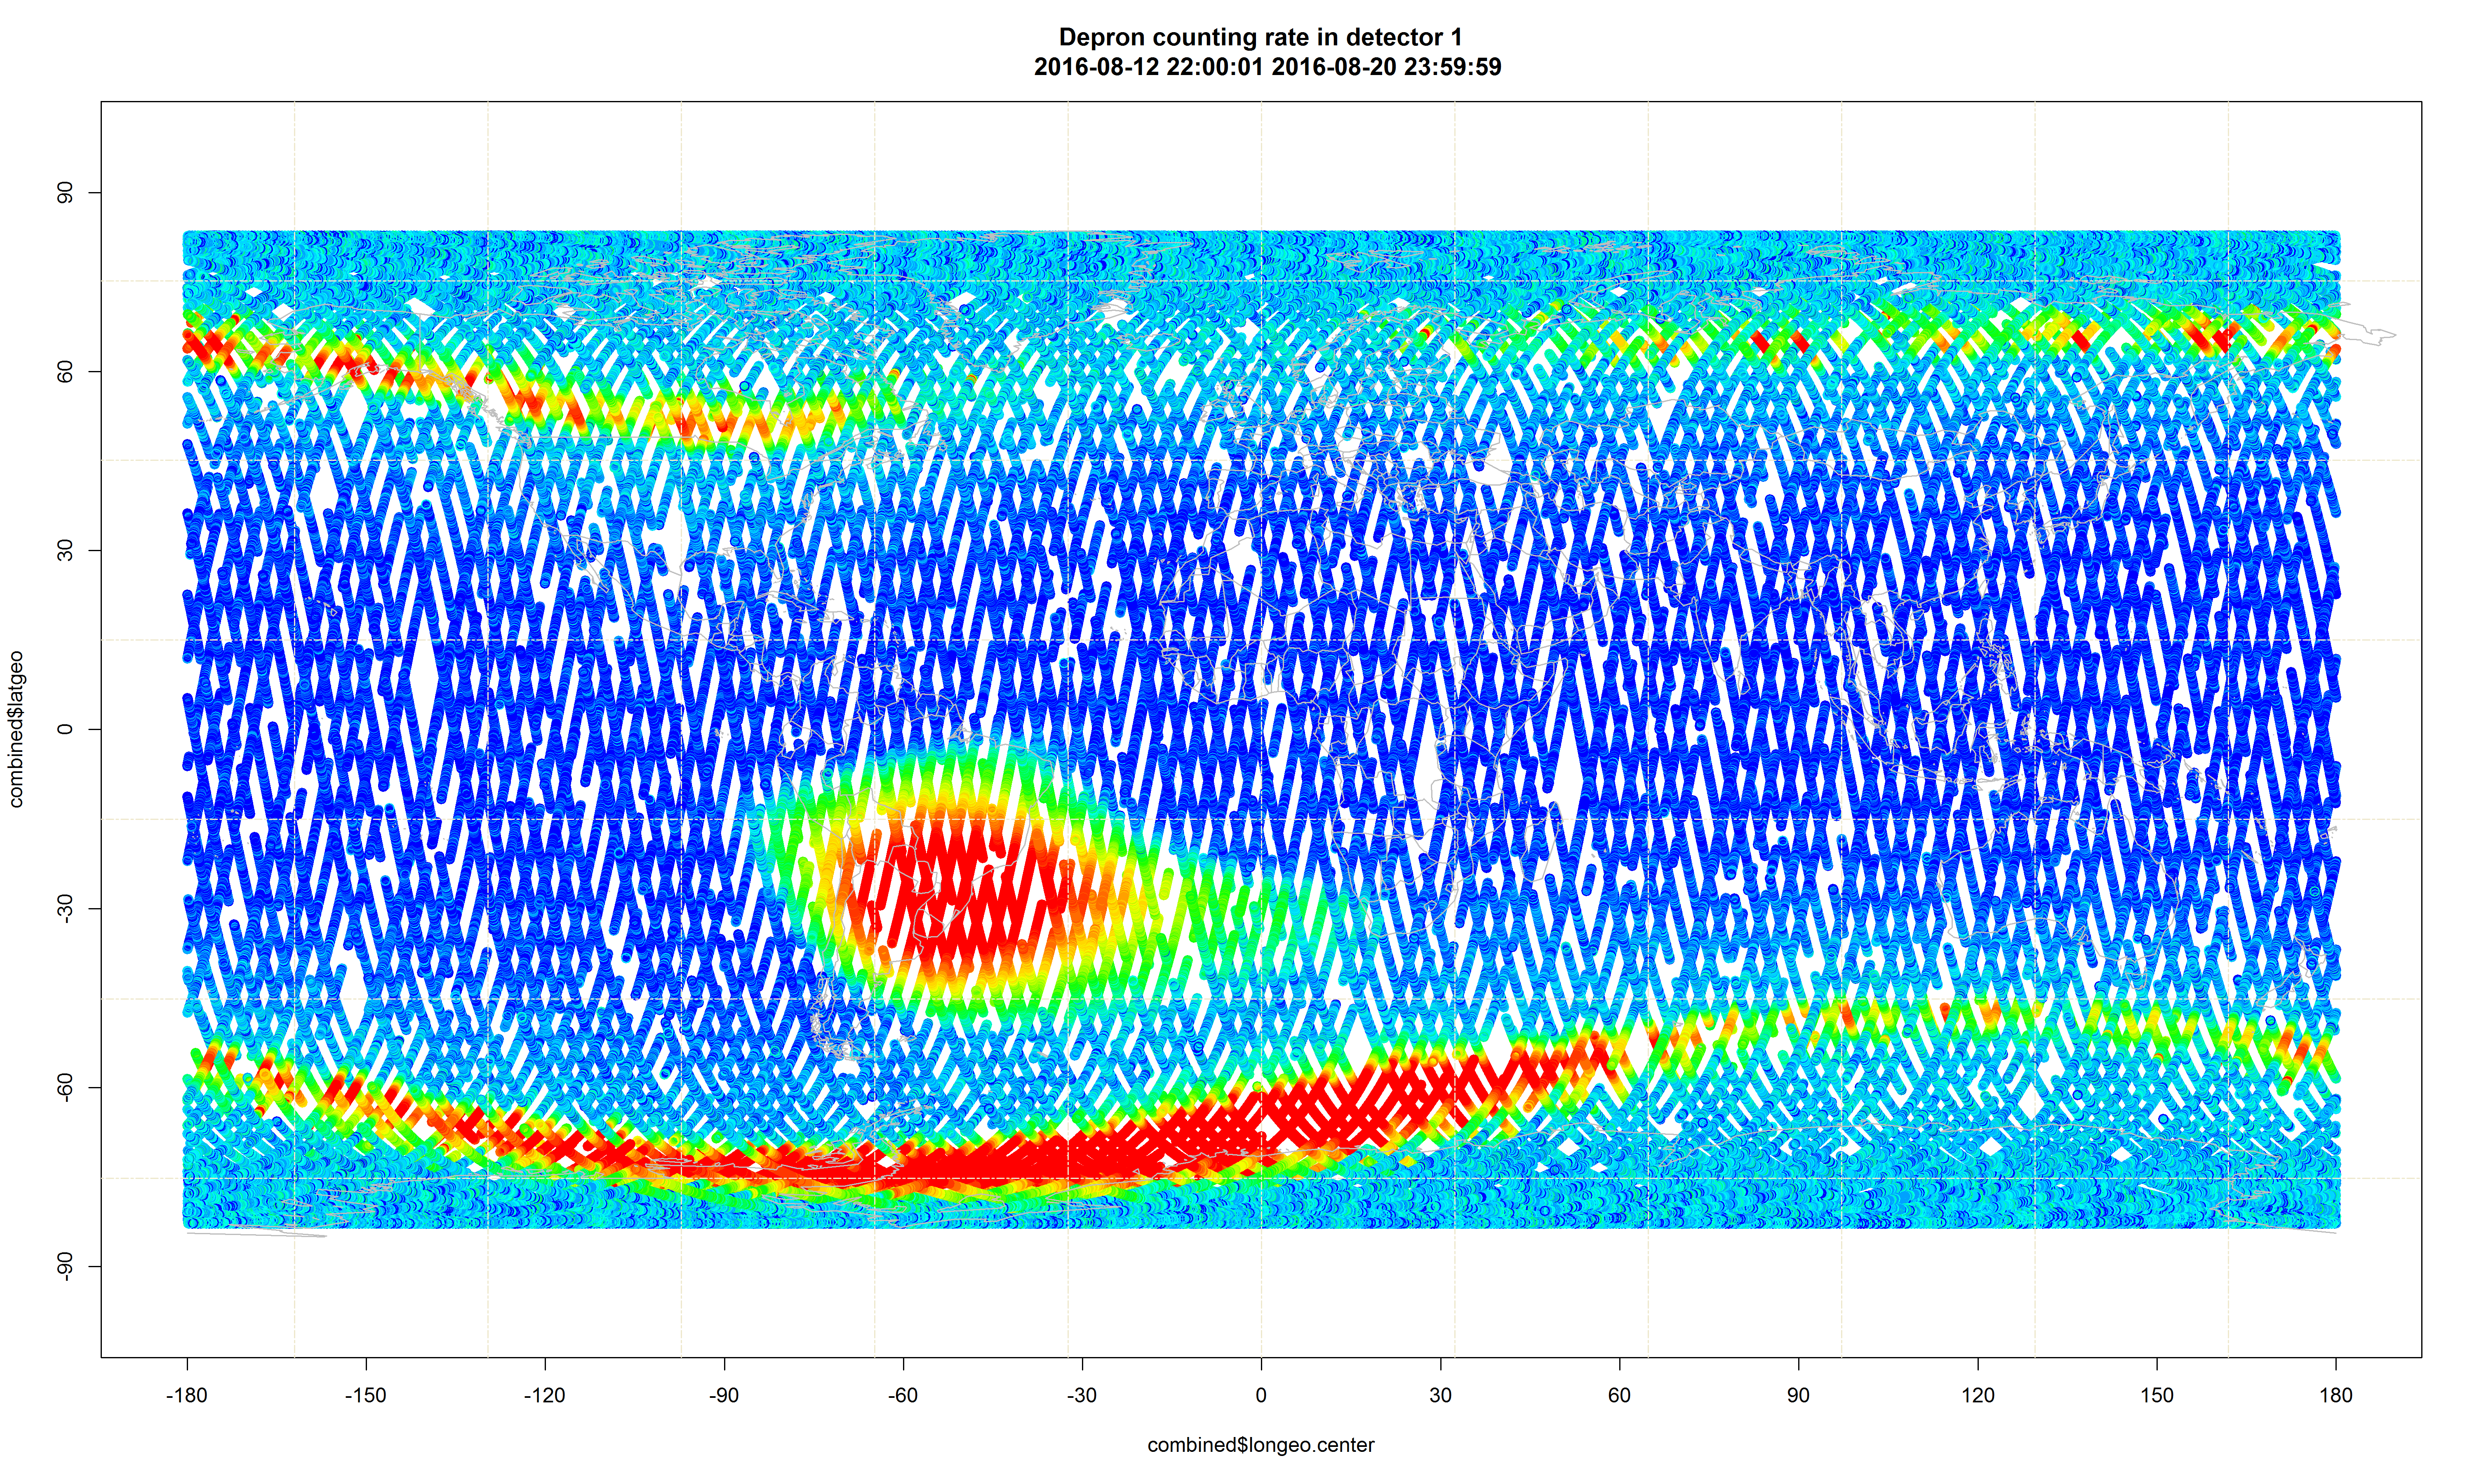
\includegraphics[width=0.79\textwidth]{images/image7}
		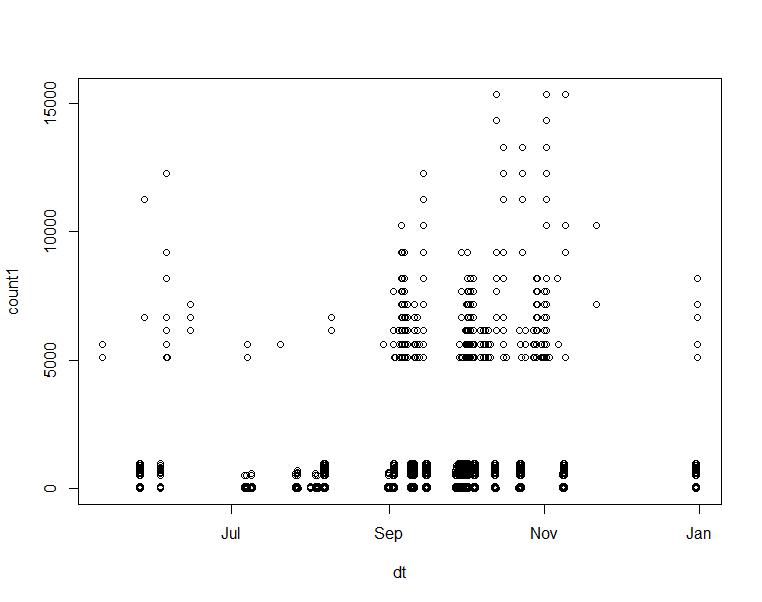
\includegraphics[width=0.2\linewidth]{images/Rplot}\\
		Longitude
	\end{center}
\end{frame}
%------------------------------------------------		
\begin{frame}
	\frametitle{\insertsection} 
	\framesubtitle{\insertsubsection}
\begin{center}
	\rotatebox{90}{
			$ B $
	}\includegraphics[width=0.79\linewidth]{images/depron_lb}	
	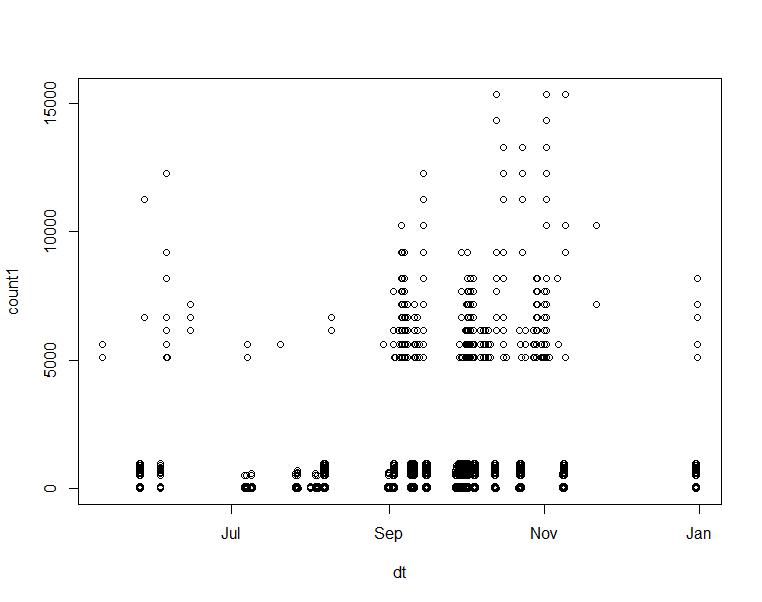
\includegraphics[width=0.2\linewidth]{images/Rplot}\\
	$ L $
\end{center}
\end{frame}

%------------------------------------------------		
\begin{frame}
	\frametitle{\insertsection} 
	\framesubtitle{\insertsubsection}
\begin{center}
	\rotatebox{90}{
			$ B $
	}\includegraphics[width=0.79\linewidth]{images/depron_lb}	
	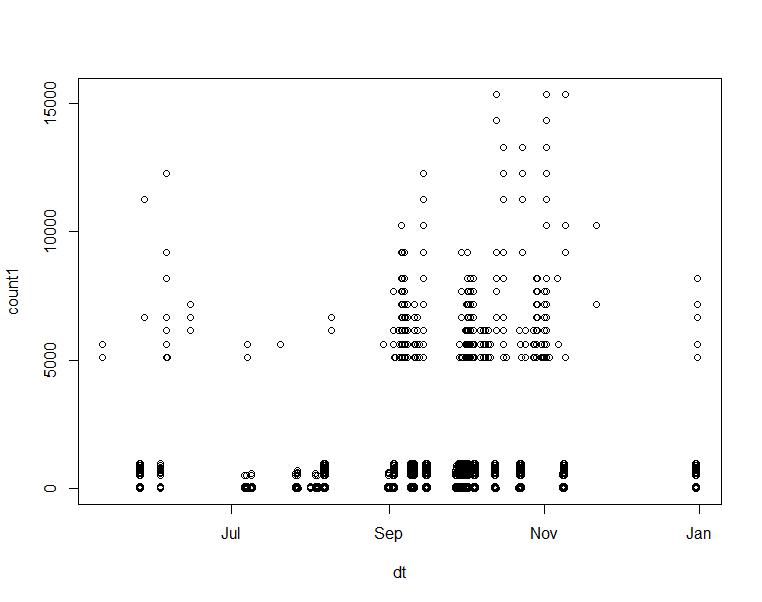
\includegraphics[width=0.2\linewidth]{images/Rplot}\\
	$ L $
\end{center}
\end{frame}
%------------------------------------------------		
\begin{frame}
	\frametitle{\insertsection} 
	\framesubtitle{\insertsubsection}
\begin{center}
\includegraphics[width=0.8\textheight]{images/depron_sec_log09-01-1600-00-00}
\end{center}
\end{frame}


%------------------------------------------------		
\begin{frame}
	\frametitle{\insertsection} 
	\framesubtitle{\insertsubsection}






	\begin{columns}[T]
		\begin{column}{.5\textwidth}
			\begin{block}{}
				\includegraphics[width=1\linewidth]{images/depron_lat_map_242}
				
				
				\includegraphics[width=1\linewidth]{images/depron_map_242}
			\end{block}
		\end{column}
		\begin{column}{.5\textwidth}
			\begin{block}{}
				
				\includegraphics[width=1\linewidth]{images/depron_sec_log08-29-1615-04-00}
											
			\end{block}
		\end{column}
	\end{columns}

\end{frame}



%\section{Normalised Radiation dynamics}
%%------------------------------------------------
%\foreach \n in {213,...,298} {%
%	\begin{frame}{Counts in detector 1 day \n}
%		\includegraphics[height=7cm]{images/hist/norm_depron_lb3d_polar\n.png}
%	\end{frame}%
%}



%\section{Normalised Radiation dynamics}
%------------------------------------------------		
%\begin{frame}
%	\frametitle{\insertsection} 
%	\framesubtitle{\insertsubsection}
%	\begin{figure}
%		\centering
%		\includegraphics[width=0.7\linewidth]{images/Graph3}
%		\caption{}
%		\label{fig:graph3}
%	\end{figure}
%\end{frame}
%------------------------------------------------			
\section{Summary}

\begin{frame}
	\begin{center}					
		\frametitle{\insertsection}
		\begin{itemize}
			\item Depron works properly register streams of charged particles and accumulated dose, taking into account the spectrum of energy release.
			\item Neutron fluxes registered
			\item Absorbed Doses per day is about 
		\end{itemize}
	\end{center}
\end{frame}

%------------------------------------------------			
\section{Future plans}

\begin{frame}
	\begin{center}					
		\frametitle{\insertsection}
		
		\begin{itemize}
			\item Dynamics of doses per day with the division of the anomaly and the contribution of the auroral zone and GCR
			
			\item According to GCR receive the latitudinal distribution of the dose rate (in L)
			
			\item The study of intensity variations  in the zone of L $ ~ $ 4-6 			
			
		\end{itemize}
	\end{center}
\end{frame}
	
%------------------------------------------------		


%\bgroup

%\usebackgroundtemplate{%
%	\tikz[overlay,remember picture] \node[opacity=0.3, at=(current page.center)] {
%	%	\includegraphics[width=\paperwidth]{images/sborka_1_3D}};
%}


%	\egroup	

\begin{frame}
	
\begin{center}
		\LARGE {Thank you for Attention!}
\end{center}
	
	Key Personalies:
	\begin{itemize}
		\item Victor Benghin
		
		\item Ivan~Zolotarev
		
		\item Oleg~Nechayev
		
		\item Alexander~Amelyushkin
		
		\item Nikolai~Vedenkin
		
		\item Vasiliy~Petrov
		
		\item M.I.~Panasyuk
		
		\item I.V.~Yashin
		
	\end{itemize}
	
	Contact email:
	brilkov@yandex.ru 
\end{frame}
			

	
